Ein monostabiler Multivibrator (auch monost. Kippstufe, Monoflop) generiert bei Triggerung einen Ausgangsimpuls definierter Länge.

\emph{Nachtriggerbare} Monoflops haben die Eigenschaft, während des aktiven
Ausgangszustandes durch ein erneutes Eingangssignal neugestartet zu werden,
wodurch sich die Ausgangsimpulsdauer verlängert. 

Monoflops können z.B. verwendet werden, um Tasterprellen zu unterdrücken,
indem sie durch den ersten Prellimpuls ausgelöst werden und dann für eine
bestimmte Zeit im aktiven Zustand bleiben, in welchem keine weiteren
Prellimpulse eine Ausgangsänderung hervorrufen können.

\begin{figure}[]
  \begin{center}
    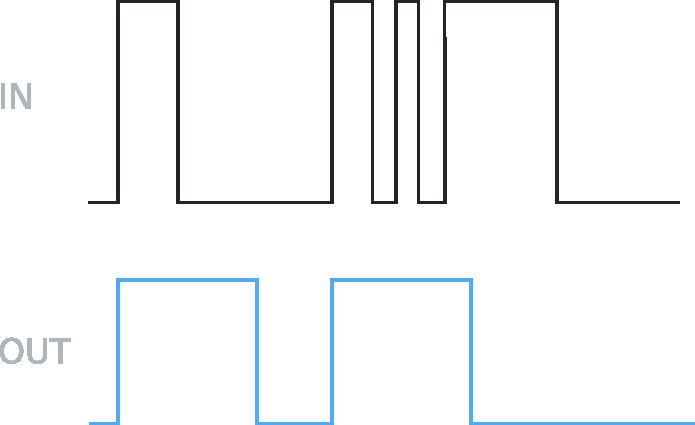
\includegraphics[width=0.382\textwidth]{VBA/2/monoop}
  \end{center}
  \caption{Beispielhafter Signalverlauf eines Monoflops}
\end{figure}